\section{INTRODUCTION}

Autonomous Vehicles are widely anticipated to alleviate road congestion through
higher throughput, improve road safety by eliminating human error, and free
drivers from the burden of driving, allowing greater productivity and/or time
for rest, along with a myriad of other foreseen benefits. The past three decades
have seen steadily increasing research efforts in developing self-driving
vehicle technology, in part fueled by advances in sensing and computing
technologies which have resulted in reduced size and price of necessary
hardware.

\begin{figure}[h]
    \centering
    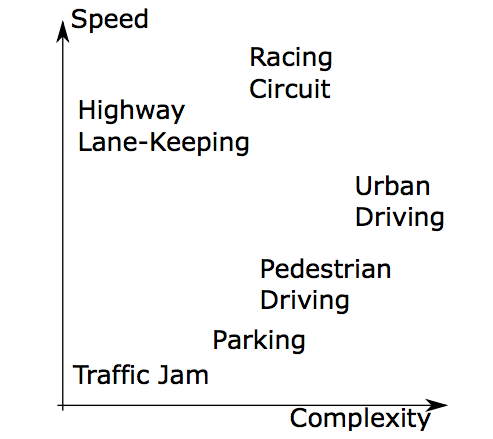
\includegraphics[width=0.5\textwidth]{speedComplexity.png}
    \caption{Complexity and operating velocity for various driving scenarios.}
    \label{fig:speedComplexity}
\end{figure}

Driving in urban environments has been of great interest to researchers due in
part to the high density of vehicles and various area-specific traffic rules
that must be obeyed. Referring to Figure \ref{fig:speedComplexity}, the problem
of urban driving is both interesting and difficult because it pushes the
research direction to address both increased operating speeds of autonomous
vehicles as well increased environmental complexity.

\subsection{History}

A future with self-driving cars was first envisioned as early as 1918, with the
idea even broadcasted over television as early as 1958. By 1988, Carnegie
Mellon’s NAVLAB vehicle was being demonstrated to perform lane-following using
camera images \cite{navlab}. Development was accelerated when several research
teams later developed more advanced driverless vehicles for competing in the
competitions organized by the Defense Advanced Research Projects Agency (DARPA).

The first, named DARPA Grand Challenge, was realized at the Mojave Desert, USA,
in 2004, and required driverless cars to navigate a 142 mi long course
throughout desert trails within a 10 h time limit. All competing cars failed
within the first few miles.

The DARPA Grand Challenge \cite{BUE07} was repeated in 2005 and required robotic
cars to navigate a 132 mi long route through flats, dry lake beds, and mountain
passes, including three narrow tunnels and more than 100 sharp left and right
turns. This competition had 23 finalists and4 cars completed the route within
the allotted time limit. The Stanford University’s car, “Stanley” \cite{THR07},
claimed first place, and the Carnegie Mellon University’s cars “Sandstorm” and
“H1ghlander”finished in second and third places, respectively.

The third competition, known as the DARPA Urban Challenge \cite{BUE09}, was held
at the former George Air Force Base, California, USA, in 2007, and required
self-driving cars to navigate a 60 mi long route throughout a simulated urban
environment, together with other self-driving and human driven cars, within a 6
h time limit. The cars had to obey California traffic rules. This competition
had 11 finalists and 6 cars completed the route within the allotted time limit.
The Carnegie Mellon University’s car, “Boss” \cite{URM08}, claimed first place,
the Stanford University’s car, “Junior” \cite{MON08}, finished in second, and
the Virginia Tech’s car, “Odin” \cite{BAC08}, came in third place. Even though
these competitions presented challenges much simpler than those typically seen
in everyday traffic, they have being hailed as milestones for the development of
self-driving cars and the research related to self-driving has since continued
at a fast pace in academic settings, but furthermore is now receiving
considerable attention in industry as well.

As research in the field of autonomous vehicles has matured, a wide variety of
impressive demonstrations have been made on full-scale vehicle platforms. Recent
studies have also been conducted to model and anticipate the social impact of
implementing autonomous Mobility-on- Demand (MoD) \cite{zhang}. The case studies
have shown that MoD system would make access to mobility more affordable and
convenient compared to traditional mobility system characterized by extensive
private vehicle ownership.

Autonomous driving on urban roads has seen tremendous progress in recent years,
with several commercial entities pushing the bounds alongside academia. Google
has perhaps the most experience in the area, having tested its fleet of
autonomous vehicles for more than 2 million miles, with expectation to soon
launch a pilot MoD service project using 100 self-driving vehicles. Tesla is
early to market their work, having already provided an autopilot feature in
their 2016 Model S cars. Uber’s mobility service has grown to upset the taxi
markets in numerous cities worldwide, and has furthermore recently indicated
plans to eventually replace all their human driven fleet with self-driving cars,
with their first self-driving vehicle pilot program already underway.
 
There are several places where automated road shuttles are in commercial
operations. Examples include deployments at Rivium Business Park, Masdar City,
and Heathrow Airport \cite{masdar}. The common feature of these operations is
that road vehicles are certified as a rail system meaning that vehicles operate
in a segregated space \cite{masdar}. This approach has been necessary due to
legal uncertainty around liability in the event of an accident involving an
autonomous vehicle. To address this, governments around the world are reviewing
and implementing new laws. Part of this process has involved extended public
trials of automated shuttles, with CityMobil and CityMobil2 being among the
largest of such projects \cite{masdar}.

To gauge the level of autonomy of self-driving cars, SAE International (formerly
simply SAE, or Society of Automotive Engineers) published a classification
system based on the amount of human driver intervention and attentiveness
required by them, in which the level of autonomy of a self-driving car may range
from level 0 (the car’s autonomy system issues warnings and may momentarily
intervene but has no sustained car control) to level 5 (no human intervention is
required in any circumstance) \cite{sae}. In this report, we focus on cars which
are equipped with an autonomy system that can be categorized as SAE level 3 or
higher

\subsection{Overview}

In this section, we present an overview of the typical architecture of the
automation system of self-driving cars and comment on the responsibilities of
the perception system, decision making system, and their subsystems.

\begin{figure}[h]
    \centering
    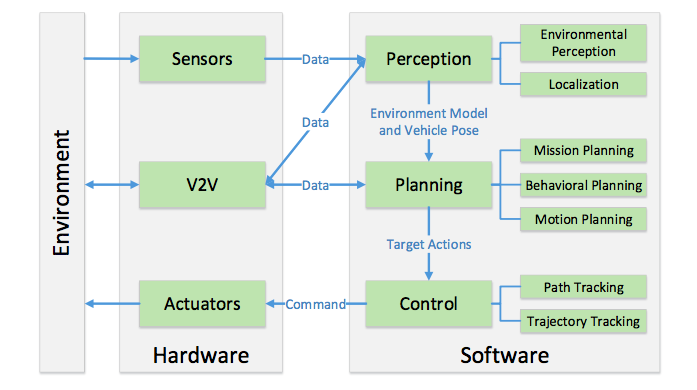
\includegraphics[width=0.9\textwidth]{systemOverview.png}
    \caption{A typical autonomous vehicle system overview.}
    \label{fig:systemOverview}
\end{figure}

Figure \ref{fig:systemOverview} and \ref{fig:caroverview} show a block diagram
of the typical architecture of the automation system of self-driving cars, where
the perception and decision making systems [PAD16] are shown as a collection of
modules of different colors. The perception system is responsible for estimating
the state of the car and for creating an internal (to the self-driving system)
representation of the environment, using data captured by on-board sensors, such
as Light Detection and Ranging (LIDAR), Radio Detection and Ranging (RADAR),
camera, Global Positioning System (GPS), Inertial Measurement Unit (IMU),
odometer, etc., and prior information about the sensors’ models, road network,
traffic rules, car dynamics, etc. The decision making system is responsible for
navigating the car from its initial position to the Final Goal defined by the
user, considering the car state and the internal representation of the
environment, as well as traffic rules and passengers’ comfort.

\begin{figure}[h]
    \centering
    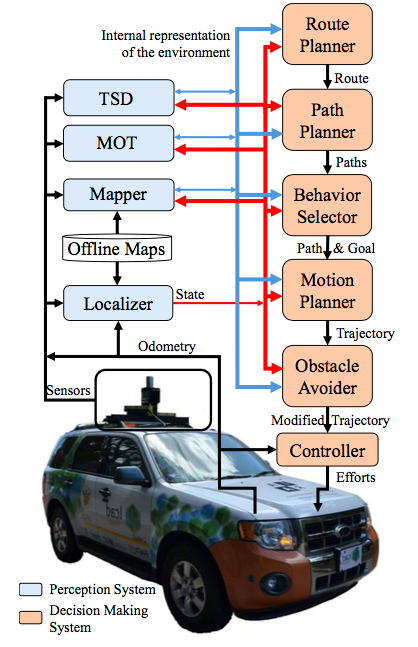
\includegraphics[height=0.5\textheight]{caroverview.png}
    \caption{Overview of the typical hierarchical architecture of self-driving cars. TSD denotes Traffic Signalization Detection and MOT, Moving Objects Tracking.}
    \label{fig:caroverview}
\end{figure}

The core competencies of an autonomous vehicle software system can be broadly
categorized into three categories, namely perception, planning, and control,
with the interactions between these competencies and the vehicle’s interactions
with the environment depicted in Figure \ref{fig:systemOverview}. Also,
Vehicle-to-Vehicle (V2V) communications can be leveraged to achieve further
improvements in areas of perception and/or planning through vehicle cooperation.

In order to navigate the car throughout the environment, the decision-making
system needs to know where the car is in it. The Localizer module (Figure
\ref{fig:caroverview}) is responsible for estimating the car state (pose, linear
velocities, angular velocities, etc.) in relation to static maps of the
environment. These static maps, (or Offline Maps, Figure \ref{fig:caroverview}),
are computed automatically before the autonomous operation, typically using the
sensors of the self-driving car itself, although manual annotations (i.e. the
position of pedestrian crossing or of traffic lights) or editing (i.e. for
removing non-static objects captured by the sensors) are usually required. A
self-driving car may use one or more different Offline Maps, such as occupancy
grid maps, remission maps, or landmark maps, for localization.

Perception refers to the ability of an autonomous system to collect information
and extract relevant knowledge from the environment. Environmental perception
refers to developing a contextual understanding of environment, such as where
obstacles are located, detection of road signs/marking, and categorizing data by
their semantic meaning. Localization refers to the ability of the robot to
determine its position with respect to the environment.

The Motion Planner module is responsible for computing a Trajectory, 𝑇, from
the current car’s state to the current Goal, which follows the Path defined by
the Behavior Selector, satisfies car’s kinematic and dynamic constraints, and
provides comfort to the passengers. A Trajectory $ T = \{c1, c2, \ldots, c|T|\} $ is
sequence of commands, $ ck = (vk, \psi k, tk) $, where $vk$ is the desired
velocity at time $k$, $\psi k$ is the desired steering angle at time $k$ and $ tk$ is
the duration of $ck$. A Trajectory takes the car from its current State to the
Goal smoothly and safely.

Finally, the control competency, refers to the robot’s ability to execute the
planned actions that have been generated by the higher level processes. It
receives the Motion Planner trajectory, eventually modified by the Obstacle
Avoider, and computes and sends Efforts commands to the actuators of the
steering wheel, throttle and brakes in order to make the car execute the
Modified Trajectory as best as the physical world allows.